\documentclass[10pt]{article}
\usepackage{iftex}
\ifPDFTeX
\usepackage[utf8]{inputenc}
\usepackage[english]{babel} %english language
\usepackage{microtype} %better kerning
\fi
\usepackage{graphicx}
\usepackage[a4paper]{geometry}
\setlength{\columnsep}{6mm}


\usepackage[backend=biber, sorting=none]{biblatex}
\addbibresource{references.bib}

\usepackage{amssymb}
\usepackage{amsfonts}
\usepackage{amsthm}
\usepackage{amsmath}
\DeclareMathOperator*{\argmax}{arg\,max}
\DeclareMathOperator*{\argmin}{arg\,min}
\usepackage{manfnt}
\usepackage{bbm}
\usepackage{mathtools}

\usepackage{caption}
\usepackage{array}
\usepackage{microtype}

\usepackage{hyperref}

\usepackage{cleveref}
\usepackage{tikz}
\usetikzlibrary{positioning, fit, backgrounds}

\theoremstyle{definition}
\newtheorem{definition}{Definition}[section]
\newtheorem{example}[definition]{Example}

\theoremstyle{plain}
\newtheorem{theorem}[definition]{Theorem}
\newtheorem{proposition}[definition]{Proposition}

\theoremstyle{remark}
\newtheorem{remark}[definition]{Remark}


\title{\Large\textbf{QuESO}\\Quantum Enhanced Seat Optimizer}

\author{Marc Breiner Sørensen}
\date{\normalsize\today}

\begin{document}
	\maketitle
	
	\begin{abstract}
	\noindent \textbf{QuESO} (Quantum Enhanced Seat Optimizer), is a quadratic unconstrained 
	binary optimization (QUBO) formulation for the office seating assignment problem. 
	The problem is cast as a weighted quadratic assignment problem (WQAP) over two graphs: 
	a flow graph encoding pairwise employee affinities and a distance graph encoding office 
	seat adjacency. The formulation accommodates an arbitrary number of rooms with 
	configurable geometry, variable employee attendance over a discrete time period, fixed 
	seat constraints, and the case where the number of employees exceeds the number of 
	available seats. The latter is handled through introduction of a null seat, rendering 
	the problem always feasible and allowing the optimizer to jointly determine seating 
	assignments and identify unassigned employees. Attendance data modulates pairwise 
	affinities to reflect shared onsite time, and a variable elimination preprocessing step 
	reduces problem size by removing absent and fixed-seat employees prior to optimization. 
	The resulting QUBO matrix is derived in closed form, with explicit expressions for all 
	matrix elements and their contributions from the objective and constraint penalty terms. 
	The formulation is solver-agnostic and is implemented in the open source package 
	\texttt{QuESO}, targeting CPU-based quantum-inspired annealers.
	\end{abstract}
	
	\newpage
	\tableofcontents
	\section{Introduction}
	We derive a \emph{Quadratic Unconstrained Binary Optimization} (QUBO) formulation for optimizing seating in the context of office spaces. The problem has equivalence with the well-known graph problem of a \textit{weighted quadratic assignment problem} (WQAP). QUBO formulations encompasses a rich class of combinatorial optimization problems that are in general known to be $\mathcal{NP}$-hard.
	
	We begin by giving a definition of QUBO problems. 
	
	\begin{definition}[QUBO]
		Let $\mathbb{B}^n$ be the \textit{n}-dimensional vector space over the binary field $\mathbb {B}$. QUBO problems are binary optimization problems that consist of finding the argument $x\in\mathbb{B}^n$, which minimizes some unconstrained pseudo-boolean function $C(x): \mathbb{B}^n\rightarrow\mathbb{R}$,
		which may be formulated as quadratic forms. 
		\begin{align}
			& \argmin_{x\in\mathbb{B}^n}\,\, C(x) \\
			& C(x) = \mathbf{x}^\top Q\, \mathbf{x}, 
		\end{align}
	\end{definition}
	An example of a vector from $\mathbb{B}^n$ is $(1, 0, 0) = 4$ for $n=3$. The matrix $Q$ is typically referred to as the QUBO matrix and it completely defines the problem. Note that due to $x_i^2 = x_i$ the diagonal of $Q$ represent linear terms. Furthermore, since the $x_i$'s are simply numbers, it is symmetric: $x_ix_j = x_jx_i = \frac12x_ix_j + \frac12x_jx_i$. Hence, there exists equivalent formulations with either symmetric or upper triangular matrices. The function $C(x)$ is often referred to as the \emph{cost function}. 
	
	In our optimization context we shall be concerned with minimizing such a cost function. The cost function encodes the information that guides our choice of permutation. 
	
	WQAP can be visualized as a graph-problem. We thus give a definition of a graph.	
	
	\begin{definition}[Graph]
		A \emph{graph} is a pair $G = (V, E)$ where $V$ is a set of \emph{vertices} (or \emph{nodes})
		and $E \subseteq \binom{V}{2}$ is a set of \emph{edges}, i.e.\ unordered pairs of distinct
		vertices. If $E$ is a multiset and self-loops $\{v,v\}$ are permitted, $G$ is called a
		\emph{multigraph}. A \emph{directed graph} (digraph) replaces $E$ with a set of ordered pairs
		$A \subseteq V \times V$, called \emph{arcs}.
	\end{definition}
	
	We do not give a formal definition of WQAP, but instead explain it in relation to the problem at hand. The WQAP consist of the following problem: given two graphs - a flow graph on entities and a distance graph on locations - find the assignment of entities to locations that maximizes flow between co-located entities. For our case this means
	\begin{itemize}
		\item \textbf{Flow graph:} employees as vertices, edge weights $P_{nm}$ - how much employees $n$ and $m$ need to be near each other.
		\item \textbf{Distance graph}: seats as nodes, edge weights $A_{sv}$ - which seats are adjacent
	\end{itemize}
	WQAP is notoriously difficult even for moderate sizes. Exhaustive enumeration of solutions is an infeasible approach in any practical scale of input sizes, which is part of the motivation for attacking it with quantum-inspired solutions rather than exact solvers.
	
	\section{Problem statement}
	In this section we pose the algebraic entities needed to set up the QUBO problem. 
	
	\subsection{Preliminaries}
	We will assume a time block $T\in\mathbb{N}$ for which to optimize the seating schedule. $T$ can be any number of integer periods, and will have an implicit unit associated with it. For example, $T=5$ may represent $5$ \emph{workdays}, such that $T$ in this case represents a workweek. We will make use of this specific assumption in the following. 
	
	Let $r\in\{1,2,\dots,R\}$, for $r,R\in\mathbb{N}$, be an enumeration of the available rooms, and $\mathcal{R}_r$ be the set of seat indices belonging to room $r$. Each room is assumed to have $n_r$ seats, such that $S = \sum_{r=1}^{R} n_r$ with $S\in\mathbb{N}$ being the total number of seats in the optimization problem. 
	
	\subsection{Problem geometry}
	
	We pose a binary matrix $A\in\mathbb{B}^{S+1 \times S+1}$ encoding the room geometry, with $A_{sv}=1$ if seats $s$ and $v$ are adjacent, for $s,v\in\{1,2,S+1\}$. There are two choices in constructing $A$. Either one may choose non-zero entries only for directly adjacent (neighbouring) seats, or one may choose non-zero entries for any combination of $s,v$ for $s,v\in \mathcal{R}_r$ for some room r. For some teams it may be necessary to enforce strict adjacency, while for other larger teams, simply seating them within the same office room is sufficient. Additionally the latter choice may be more convenient for smaller room sizes. In any case the particular realization of $A$ in the end depends on the rooms that are part of the optimization task. 
	
	$A_{sv}$ is equivalent to an adjacency matrix for a graph, where each room is a partition into disjoint subgraphs indexed by $r$ with vertex labels from the set $\mathcal{R}_r$, such that joining disjoint subgraphs denoted by $G_i = \left(\mathcal{R}_i, \{A_{sv}|s,v\in \mathcal{R}_i\}\right)$ as $G = \sqcup_i G_i$ (the disjoint union of subgraphs) produces a graph which represents the problem at hand.
		
	We also note that since $A$ has equivalence to a graph adjacency matrix, conventionally $A_{sv} = A_{sv}$ since the graph is undirected. This implies a symmetric tensor. We, however, choose to represent the tensor by an upper triangular matrix representation for interpretative and algorithmic purposes, even though the graph representing our problem is undirected in the strict sense. From this we additionally choose the convention that $A_{ss = 0} \forall s$, since this self-adjacency will be shown to relate to self-affinity that in turn also rewards employees seated at the same desk, for reasons that will be clear later. Additionally this slightly reduces the density of the resulting QUBO matrix, which is marginally better for solvers.
	
	The matrix representation of $A$ will show geometric structures pertaining to this graph such as triangles and disjointedness.
	
	We now present an example with $R=2, S=8, \mathcal{R}_1=\{1,2,3,4,5\}, \mathcal{R}_2=\{6,7,8\}$ for which the matrix representation of $A$ is given by
	\begin{equation}
		A = \begin{bmatrix}
			0 & 1 & 1 & 0 & 0 & 0 & 0 & 0 & 0 \\
			0 & 0 & 1 & 0 & 0 & 0 & 0 & 0 & 0 \\
			0 & 0 & 0 & 1 & 1 & 0 & 0 & 0 & 0 \\
			0 & 0 & 0 & 0 & 1 & 0 & 0 & 0 & 0 \\
			0 & 0 & 0 & 0 & 0 & 0 & 0 & 0 & 0 \\
			0 & 0 & 0 & 0 & 0 & 0 & 1 & 1 & 0 \\
			0 & 0 & 0 & 0 & 0 & 0 & 0 & 1 & 0 \\
			0 & 0 & 0 & 0 & 0 & 0 & 0 & 0 & 0 \\
			0 & 0 & 0 & 0 & 0 & 0 & 0 & 0 & 0 
		\end{bmatrix},
	\end{equation}
	which, as noted above, displays geoetric properties of the graph such as the two triangles, and a block structure displaying the disjointedness. This $A$ matrix encodes the problem represented by the graph in figure \ref{fig:G}.
	\begin{figure}[h!]
		\centering
			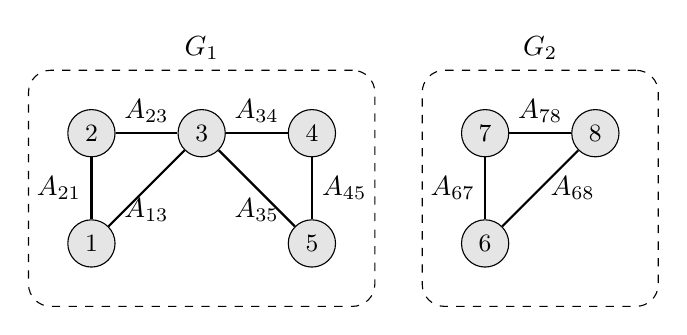
\begin{tikzpicture}[
				node/.style={draw, circle, fill=gray!20, minimum size=0.6cm, font=\small},
				every edge/.style={draw, thick},
				]
				
				%% ── Left graph (nodes 1–5) ─────────────────────────────────────────────
				\node[node] (n1) at (0,-1.4) {1};
				\node[node] (n2) at (0,0)    {2};
				\node[node] (n3) at (1.4,0)  {3};
				\node[node] (n4) at (2.8,0)  {4};
				\node[node] (n5) at (2.8,-1.4) {5};
				
				\draw[thick] (n1) -- node[below] {$A_{13}$}(n3);
				\draw[thick] (n2) -- node[above] {$A_{23}$}(n3);
				\draw[thick] (n3) -- node[above] {$A_{34}$}(n4);
				\draw[thick] (n4) -- node[right] {$A_{45}$}(n5);
				\draw[thick] (n2) -- node[left]  {$A_{21}$}(n1);
				\draw[thick] (n3) -- node[below] {$A_{35}$}(n5);
				
				\begin{scope}[on background layer]
					\node[draw, rounded corners=8pt, dashed,
					fit=(n1)(n2)(n3)(n4)(n5),
					inner sep=14pt,
					label=above:{$G_1$}] (box1) {};
				\end{scope}
				
				%% ── Right graph (nodes 6–8) ────────────────────────────────────────────
				\node[node] (n7) at (5,0)    {7};
				\node[node] (n8) at (6.4,0)  {8};
				\node[node] (n6) at (5,-1.4) {6};
				
				\draw[thick] (n7) -- node[above] {$A_{78}$}(n8);
				\draw[thick] (n7) -- node[left] {$A_{67}$}(n6);
				\draw[thick] (n8) -- node[right] {$A_{68}$}(n6);
				
				\begin{scope}[on background layer]
					\node[draw, rounded corners=8pt, dashed,
					fit=(n6)(n7)(n8),
					inner sep=14pt,
					label=above:{$G_2$}] (box2) {};
				\end{scope}
				
			\end{tikzpicture}
			\caption{Room geometry from the example represented as two disjoint subgraphs $G_i=(V_i, E_i)$. }
			\label{fig:G}
		\end{figure}
		If one does not care about immediate adjacency of seats but only whether seats are within the same room, this corresponds to forming the fully connected graph instead, which results in several additional non-zero elements in the matrix representation of $A$ and corresponds to a relaxation of the optimization problem.
	
	
	
	\subsection{The assignment matrix}
	Given $N\in\mathbb{N}$ employees to be seated, we may construct a binary matrix $X\in \mathbb{B}^{N\times S+1}$ of size $N \times S+1$, with indices $n,s\in\mathbb{N}$ representing respectively employees and seats, such that $X_{ns} = 1$ denotes that employee $n$ is assigned to seat $s$ for the week. Note that while $n\in\{1,2,\dots,N\}$ the seat index runs up to $S+1$ as $s\in\{1,2,\dots,S+1\}$ to allow an assignment to a "null" seat (no seat), represented by the value $s = S+1$ such that $X_{n(S+1)}=1$ denotes that employee $n$ was not assigned to any seat during $T$, which might be the case if $N > S$ in which case no complete assignment of all employees is possible. 
	\begin{equation}
		X = \overbrace{
			\begin{bmatrix}
				X_{11} & \cdots & X_{1(S+1)} \\
				\vdots & \ddots & \vdots \\
				X_{N1} & \cdots & X_{N(S+1)}
			\end{bmatrix}
		}^{\displaystyle S+1}
		\left.
		\vphantom{
			\begin{bmatrix}
				X_{11} \\ \vdots \\ X_{N1}
			\end{bmatrix}
		}
		\right\} N
	\end{equation}
	$X$ is a rank-2 tensor with a block form as
	\begin{equation}
		X = \begin{bmatrix}
			\begin{bmatrix}
				X_{11} & \cdots & X_{1(S+1)} \\
			\end{bmatrix}\\
			\vdots \\¨
			\begin{bmatrix}
				X_{i1} & \cdots & X_{i(S+1)}
			\end{bmatrix}\\
			\vdots\\
			\begin{bmatrix}
				X_{N1} & \cdots & X_{N(S+1)}
			\end{bmatrix}\\
		\end{bmatrix},
	\end{equation}
	such that each row of $X$ is a one-hot encoded block (vector) of length $S+1$, with the $i$'th entry being set to $1$ and all other being $0$. This structure ensures that every employee is  assigned at most one seat.
	Consider an example with $N=6, S=4$ - so five employees to be assigned to just four seats. We may write the matrix as
	\begin{equation}
		X = \begin{bmatrix}
				0 & 0 & 0 & 1 & 0 \\
				1 & 0 & 0 & 0 & 0\\
				0 & 0 & 1 & 0 & 0\\
				0 & 0 & 0 & 0 & 1\\
				0 & 1 & 0 & 0 & 0\\
				0 & 0 & 0 & 0 & 1\\
			\end{bmatrix},
	\end{equation}
	which represents an assignment where employee 1 sits at seat 4, employee 2 sits at seat 1, employee 3 sits at seat 3, employee 5 sits at seat 2 and employees 4 and 6 have no seats for the week.
	
	Notice also the structure of the matrix. Excluding the last column, each column only has at most one non-zero entry, while each of the rows have exactly one non-zero entry. This particular structure will be enforced with constraints to be defined below.
	If every seat were filled (i.e. $N=M$ and no null assignments), $X$ would be a permutation matrix, which is a special case of an orthogonal matrix since $XX^T = I$ and $X^TX=I$. In our relaxed rectangular case ($N\times(M+1)$, with possible null assignments and empty seats), $X$ is a doubly stochastic matrix in structure. More precisely it belongs to the set of partial permutation matrices. In linear algebra terms, each row of $X$ is a standard basis vector $e_k\in\{0,1\}^{S+1}$, where the position of the 1 indicates the assigned seat, and seats form an orthonormal basis with representation $e_k$. 
	
	\subsection{Employee attendance}
	In finding the right assignment of seats, we wish to consider the attendance of a given employee within the time period $T$. For $T$ in units of days, we wish to attribute greater weight to those employees that are present the most days. Employees may be sick, have scheduled time off, vacation, or be working from home. We pose the matrix $W\in\mathbb{B}^{N \times T}$, where $T=5$ for a workweek. $W_{nt} = 1$ if employee $n$ is present at the office on day $t,$ for $t\in\{1,\dots,T\}$. We continue our example from before with $N=6, T=5$.
	
	\begin{equation}
		W = \begin{bmatrix}
			1 & 1 & 1 & 1 & 1 \\
			1 & 1 & 1 & 0 & 0 \\
			1 & 1 & 1 & 0 & 0 \\
			1 & 0 & 1 & 1 & 1 \\
			1 & 1 & 1 & 1 & 1 \\
			1 & 1 & 1 & 1 & 1 
		\end{bmatrix}
	\end{equation}
	representing the case where employees 1, 5 and 6 are present at the office every day of the week, while employees 2 and 3 are off-site Thursday and Friday, and employee 4 is off-site on Tuesday.
	
	\subsection{Employee relations}
	Probably most importantly, our solution must take into account the necessity for two or more employees to be seated adjacently. We represent these relationships with the matrix $P\in\mathbb{B}^{N\times N}$, where $P_{nm} = C$ is equal to some constant $C\in\mathbb{R}$, which describes the degree of necessity, or affinity, of employee $n$ to be seated next to employee $m$. 
	
	Note that $P$ is equivalent to a digraph $G$ representing employee relations. In this sense $P$ is a weighted adjacency matrix where in general $P_{nm} \neq P_{mn}$ since the two employees may not hold the same affinity for one another. 
	Expanding on our running example for $N = 6$ a realization of $P$ could be (here denoting only $P_{nm}$ for non-zero entries).
	
	\begin{equation}
		P = \begin{bmatrix}
			0  		& P_{12} & P_{13} & 0      & 0 		& 0			\\	
			P_{21} 	& 0      & P_{23} & 0      & 0 		& P_{26} 	\\
			P_{31} 	& P_{32} & 0      & P_{34} & P_{35} & P_{36}	\\
			0 		& 0	     & P_{43} & 0      & 0 		& 0			\\
			0 		& 0		 & P_{53} & 0      & 0 		& 0			\\
			0 		& P_{62} & P_{63} & 0      & 0 		& 0			\\
		\end{bmatrix}
	\end{equation}
	which corresponds to the graph
	\begin{figure}[h!]
		\centering
		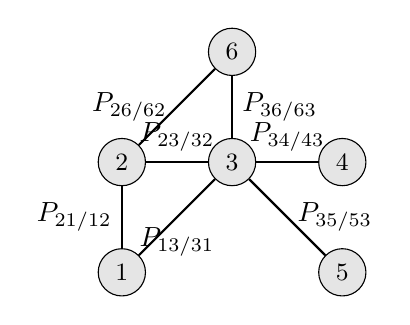
\begin{tikzpicture}[
			node/.style={draw, circle, fill=gray!20, minimum size=0.6cm, font=\small},
			every edge/.style={draw, thick},
			]
			
			%% ── Left graph (nodes 1–5) ─────────────────────────────────────────────
			\node[node] (n1) at (0,-1.4) {1};
			\node[node] (n2) at (0,0)    {2};
			\node[node] (n3) at (1.4,0)  {3};
			\node[node] (n4) at (2.8,0)  {4};
			\node[node] (n5) at (2.8,-1.4) {5};
			\node[node] (n6) at (1.4,1.4) {6};
			
			\draw[thick] (n1) -- node[below] {$P_{13/31}$}(n3);
			\draw[thick] (n2) -- node[above] {$P_{23/32}$}(n3);
			\draw[thick] (n3) -- node[above] {$P_{34/43}$}(n4);
			\draw[thick] (n2) -- node[left]  {$P_{21/12}$}(n1);
			\draw[thick] (n3) -- node[right] {$P_{35/53}$}(n5);
			\draw[thick] (n3) -- node[right] {$P_{36/63}$}(n6);
			\draw[thick] (n2) -- node[left] {$P_{26/62}$}(n6);
			
			
		\end{tikzpicture}
		\caption{Room geometry from the example represented as two disjoint subgraphs $G_i=(V_i, E_i)$. }
		\label{fig:G}
	\end{figure}
	
	\subsection{Fixed seating}
	Some employees might, for one reason or the other, require a fixed seat during the period of optimization. Such a constraint may be enforced on the problem via introduction of a binary matrix $F\in\mathbb{B}^{N\times S}$ where $F_{ns} = 1$ means employee $n$ must be seated at seat $s$. We continue with our running example for $N=6, S=4, T=5$.
	\begin{equation}
		F = \begin{bmatrix}
			0 & 0 & 0 & 0 \\
			0 & 0 & 0 & 0 \\
			0 & 1 & 0 & 0 \\
			0 & 0 & 0 & 0 \\
			0 & 0 & 0 & 0 \\
			0 & 0 & 0 & 1
		\end{bmatrix}
	\end{equation}
	representing the case where employee 3 must be assigned to seat 2, while employee 6 must be assigned to seat 4.

	
	\section{The full QUBO formulation}
	We now have all of the components that define our problem. In order to exploit algorithms to solve QUBO problems we simply have left to put the pieces together in a formulation of the form
	\begin{equation}
		\argmin_{x\in\mathbb{B}^n} x^T Q x.
	\end{equation} 
	If we begin by vectorizing $X$, by flattening it into a $1D$-array, and identify the QUBO matrix
	\begin{equation}
		Q = - \sum_{nmsv}\tilde{P}_{nm} A_{sv}\cdot e_{ns} e_{mv}^T + \lambda_1 P_1 + \lambda_2 P_2 + \lambda_3 P_3,
	\end{equation}
	where the augmented intra-day affinity matrix $\tilde{P}$ is
	\begin{equation}
		\tilde{P}_{nm} = P_{nm}\sum_{t=1}^T W_{nt}W_{mt},
	\end{equation}
	and the penalty terms, that enforce our identified constraints are given by
	\begin{align}
		P_{\text{row}} &= \sum_{n=1}^{N} \left(1 - \sum_{s=1}^{S+1} X_{ns}\right)^2\\
		P_{\text{col}} &= \sum_{s=1}^{S} \sum_{n < m} X_{ns} X_{ms}\\
		P_{\text{fixed}} &= \sum_{n,s} F_{ns}(1 - X_{ns})^2 
		+ \sum_{n} \mathbf{1}[\exists s : F_{ns} = 1] \sum_{v \neq s} X_{nv}^2,
	\end{align} 
	then we have a valid QUBO form. We unpack these contributions in the following. Before we do this, we give an overview of using the technique of \textit{variable elimination} to reduce the complexity of the QUBO before annealing.	
	
	\section{Variable Elimination}
	
	Before constructing the QUBO matrix, we may reduce the size of the problem by 
	identifying variables whose values are known \textit{a priori}, and substituting 
	these known values directly into the objective and constraint terms. This procedure 
	is known as \emph{variable elimination}, and it reduces both the number of free 
	variables and the size of the resulting QUBO matrix, which is beneficial for solver 
	performance.
	
	\subsection{Elimination of absent employees}
	
	Recall the modulated affinity matrix
	\begin{equation}
		\tilde{P}_{nm} = P_{nm} \sum_{t=1}^{T} W_{nt} W_{mt}.
	\end{equation}
	If employee $n$ has no attendance during the period $T$, i.e. $\sum_t W_{nt} = 0$, 
	then $\tilde{P}_{nm} = 0$ for all $m$. Employee $n$ contributes nothing to the 
	affinity objective regardless of their seat assignment, and assigning them a real 
	seat wastes a seat that could be allocated to an attending employee. We therefore 
	set $X_{n(S+1)} = 1$ and $X_{ns} = 0$ for all $s \leq S$, and remove all variables 
	$\{X_{ns}\}_{s=1}^{S+1}$ from the problem entirely.
	
	\subsection{Elimination of fixed-seat employees}
	
	Suppose employee $n^*$ has a fixed seat assignment $s^*$, i.e. $F_{n^* s^*} = 1$ for some 
	$s^* \leq S, n^* \leq N$. Then we know with certainty that
	\begin{equation}
		X_{n^* s^*} = 1, \qquad X_{n^* s} = 0 \;\forall s \neq s^*, \qquad 
		X_{n s^*} = 0 \;\forall n \neq n^*.
	\end{equation}
	We substitute these values directly into the objective. Consider the affinity terms 
	involving employee $n^*$:
	\begin{equation}
		-\sum_{m, s, v} \tilde{P}_{n^* m} A_{s^* v} X_{n^* s^*} X_{m v} 
		= -\sum_{m, v} \tilde{P}_{n^* m} A_{s^* v} X_{m v},
	\end{equation}
	where we have substituted $X_{n^* s^*} = 1$. This term, which was previously 
	quadratic in $X$, is now \emph{linear} in $X_{mv}$. In QUBO notation, linear 
	terms correspond to diagonal entries of the QUBO matrix $Q$, since 
	$x_\mu^2 = x_\mu$ for binary variables. Specifically, for each active employee $m$ 
	and each seat $v$, the value $-\tilde{P}_{n^* m} A_{s^* v}$ is added to the 
	diagonal entry $Q_{\mu\mu}$ where $\mu$ is the flattened index corresponding to 
	$(m, v)$, which holds info about other employees "\textit{m}" seated next to $n^*$ (if adjacent).
	
	This means that fixed-seat employees are removed as decision variables — they do 
	not appear as rows or columns in the reduced QUBO matrix — yet their affinity 
	relationships with active employees are preserved as linear biases on the active 
	employees' seat variables. The column constraint for seat $s^*$ is also trivially 
	satisfied and may be dropped from $P_\text{col}$.
	
	\subsection{The reduced problem}
	
	Let $\mathcal{N}_\text{active} \subseteq \{1, \dots, N\}$ denote the set of 
	employees remaining after both elimination steps, with $N_\text{active} = 
	|\mathcal{N}_\text{active}|$. The reduced assignment matrix $\hat{X} \in 
	\mathbb{B}^{N_\text{active} \times (S+1)}$ contains only the rows corresponding 
	to active employees, and the reduced QUBO matrix has dimensions
	\begin{equation}
	Q \in \mathbb{R}^{N_\text{active}(S+1) \times N_\text{active}(S+1)}.
	\end{equation}
	The index mapping $\mu = n \cdot (S+1) + s$ relates each flattened variable 
	$x_\mu$ to the pair $(n, s)$ in the reduced problem. A bookkeeping structure 
	records the correspondence between reduced indices and original employee 
	identifiers, enabling the solver output to be translated back to the full employee 
	set after optimization:
	\begin{equation}
	\texttt{employee\_index\_map} = \begin{cases}
		\texttt{no\_attendance} & \{n : \sum_t W_{nt} = 0\} \\
		\texttt{pre\_fixed} & \{n \mapsto s^* : F_{ns^*} = 1\} \\
		\texttt{active} & \{\hat{n} \mapsto n : n \in \mathcal{N}_\text{active}\}
	\end{cases}
	\end{equation}
	where $\hat{n}$ denotes the reduced index of an active employee.
	
	\subsection{Linear bias from fixed employees}
	
	The full set of linear bias corrections from all fixed-seat employees is collected 
	before constructing the QUBO. For each fixed employee $n^* \in \texttt{pre\_fixed}$ 
	with assigned seat $s^*$, and for each active employee $\hat{n}$ with original index 
	$n$, the diagonal bias is
	\begin{equation}
	\Delta Q_{\mu\mu} = -\tilde{P}_{n^* m} A_{s^* v}, 
	\qquad \mu = \hat{n} \cdot (S+1) + v,
	\end{equation}
	summed over all fixed employees $n^*$. These corrections are added to the diagonal 
	of $Q$ after the quadratic terms have been assembled.
	
	\section{Structure of the matrix elements}
	
	The QUBO matrix $Q_{nmsv}$ is most naturally understood as a rank-4 tensor 
	before flattening. Given the double index structure of $X_{ns}$, we write the 
	matrix elements as $Q_{ns, mv}$, which after applying the flattening map 
	$\mu(n,s) = n \cdot (S+1) + s$ correspond to $Q_{\mu(n,s),\mu(m,v)}$. 
	The full matrix element is
	
	\begin{equation}
		Q_{ns,mv} = -\tilde{P}_{nm} A_{sv} 
		+ \lambda_1 [P_{\text{row}}]_{ns,mv} 
		+ \lambda_2 [P_{\text{col}}]_{ns,mv},
	\end{equation}
	
	and we now expand each contribution.
	
	\subsection{Affinity term}
	The affinity contribution is simply
	\begin{equation}
		-\tilde{P}_{nm} A_{sv},
	\end{equation}
	which is non-zero only when employees $n$ and $m$ have nonzero affinity and seats 
	$s$ and $v$ are adjacent. This term is purely off-diagonal in the employee indices 
	when $n \neq m$.
	
	\subsection{Row penalty}
	Every employee must be assigned to exactly one seat (or the null seat), giving
	an equality constraint. EExpanding $P_\text{row} = \sum_n \left(1 - \sum_s X_{ns}\right)^2$ for a fixed employee $n$ yields
	\begin{align}
		\left(1 - \sum_s X_{ns}\right)^2
		&= 1 - 2\sum_s X_{ns} + \sum_s\sum_{v} X_{ns}X_{nv} \notag \\
		&= 1 - 2\sum_s X_{ns} + \sum_s X_{ns}^2 + \sum_{s \neq v} X_{ns}X_{nv} \notag \\
		&= 1 - \sum_s X_{ns} + \sum_{s \neq v} X_{ns}X_{nv},
	\end{align}
	where we used $X_{ns}^2 = X_{ns}$ for binary variables. Or the full form given as
	
	\begin{equation}
		P_\text{row} = \sum_n \left(1 - 2\sum_s X_{ns} + \sum_s \sum_{v} X_{ns} X_{nv}\right).
	\end{equation}
	The contributions to the
	QUBO matrix are therefore a diagonal term of $-1$ per variable and a quadratic
	coupling of $+1$ between any two seats of the same employee. Crucially, different
	employees are never coupled by $P_\text{row}$, since the sum over $n$ is independent.
	
	
	\subsection{Column penalty}
	One might expect the column penalty to take the analogous squared form
	\begin{equation}
		P_\text{col} \stackrel{?}{=} \sum_{s=1}^{S} \left(1 - \sum_n X_{ns}\right)^2,
	\end{equation}
	enforcing that each seat is occupied by exactly one employee. This is however
	incorrect for two reasons. First, if $N < S$ or after variable elimination reduces
	the active employee count, seats may legitimately be unoccupied, and the squared
	form would penalize valid empty-seat configurations. Second, the constraint is
	fundamentally an inequality: no seat may be shared by more than one employee, rather than the equality required by the row constraint. The correct formulation is therefore
	\begin{equation}
		P_\text{col} = \sum_{s=1}^{S} \sum_{n < m} X_{ns} X_{ms},
	\end{equation}
	which contributes $+1$ for every pair of employees assigned to the same real seat
	and zero otherwise, with no linear term since empty seats are not penalized.
	The null seat $s = S+1$ is excluded from the sum entirely, as arbitrarily many
	employees may be assigned to it.
	
	\subsection{Diagonal elements}
	Collecting all contributions to the diagonal $\mu = \mu(n,s)$, i.e. $n=m, s=v$:
	\begin{equation}
		Q_{\mu\mu} = -\tilde{P}_{nn} A_{ss} - \lambda_1 + \Delta Q_{\mu\mu},
	\end{equation}
	where $A_{ss} = 0$ by convention and $\tilde{P}_{nn}$ encodes self-affinity, 
	which is typically zero. The $-\lambda_1$ term arises from the linear part of 
	$P_\text{row}$, and $\Delta Q_{\mu\mu}$ collects any linear bias from fixed-seat 
	employees as described in the previous section. The diagonal therefore simplifies to
	\begin{equation}
		Q_{\mu\mu} = -\lambda_1 + \Delta Q_{\mu\mu}.
	\end{equation}
	
	\subsection{Summary}
	The full element structure is collected in Table~\ref{tab:qubo_elements}.
	
	\begin{table}[h!]
		\centering
		\begin{tabular}{llll}
			\hline
			Condition & $n=m$ & $s=v$ & $Q_{ns,mv}$ \\
			\hline
			Diagonal & \checkmark & \checkmark & $-\lambda_1 + \Delta Q_{\mu\mu}$ \\
			Same employee, different seats & \checkmark & $\times$ & $+\lambda_1 - \tilde{P}_{nn}A_{sv}$ \\
			Different employees, same seat & $\times$ & \checkmark & $+\lambda_2 - \tilde{P}_{nm}A_{ss}$ \\
			Different employees, different seats & $\times$ & $\times$ & $-\tilde{P}_{nm}A_{sv}$ \\
			\hline
		\end{tabular}
		\caption{Structure of the QUBO matrix elements $Q_{ns,mv}$ by index case. 
			Note $A_{ss}=0$ by convention, simplifying the third row to $+\lambda_2$.}
		\label{tab:qubo_elements}
	\end{table}
	
\end{document}
